\section{Improved Client GUI}
Inspired by the recently completed World Chess Championship and our group name, IPM (abbreviation of Introductory Programming, group M), being a pun on IBM. We decided to implement a visual style honouring the late, great chess computer, Deep Blue.

The site has a simple mobile-first layout. A dynamic background resembling the inner workings of a sophisticated AI fills the screen. In front are simple form elements with a retro, monospace font (Figure \ref{fig:gui:noResults}). A search is carried out both when clicking on the search button and when pressing \textit{Enter} while focus is in the search field. 

\begin{figure} [h]
	\centering
	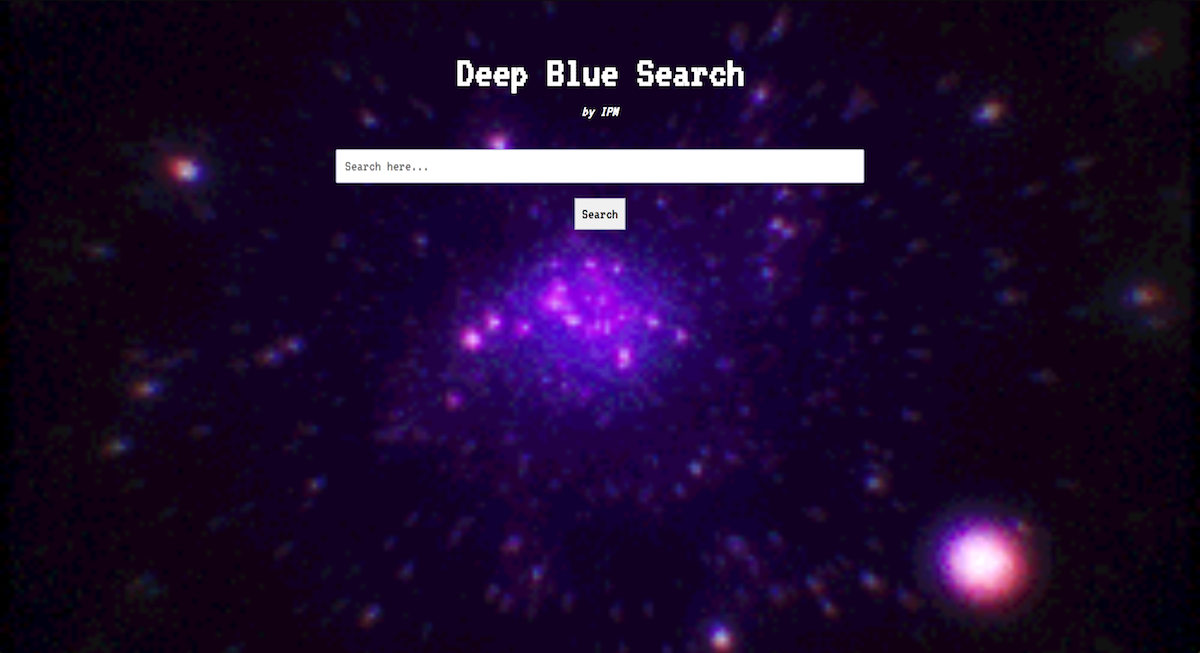
\includegraphics[width=\textwidth]{graphics/gui-noResults.png}
	\caption{The GUI before a search is conducted}
	\label{fig:gui:noResults}
\end{figure}

When a search has been completed, a few details are displayed: The amount of websites retrieved, the time it took, and a tip of the hat to Garry Kasparov (see implementation in Listing \ref{lst:kasparov}). Below, results are displayed with a simple preview (Figure \ref{fig:gui:results}). The preview is generated on the front-end (Listing \ref{lst:preview}).

\begin{lstlisting}[language=Java,
	caption={The Kasparov Algorithm},
	label={lst:kasparov}]
// Returns a random response regarding the activities of Garry Kasparov
function kasparov(responseSize){
	var responses = ["Kasparov is still computing", "Kasparov is contemplating e4", "Kasparov retrieved none", "Kasparov regrets the Sicilian Defense"];

	if(responseSize > 0){
		return responses[Math.floor(Math.random() * responses.length)];
	} else {
		return "Kasparov gloats excessively"
	}
}
\end{lstlisting}

\begin{lstlisting}[language=Java,
	caption={Preview generation},
	label={lst:preview}]
const regex = /"|\[|\]/gm;

// Convert the JSON data to a string, replace commas with spaces 
// and the special characters defined by the regular expression by the empty string. 
// Finally, get the substring from index 0 to 140

var preview = JSON.stringify(value.words).replace(/,/g, " ").replace(regex, "").substring(0, 140);
\end{lstlisting}

\begin{figure}[h]
	\centering
	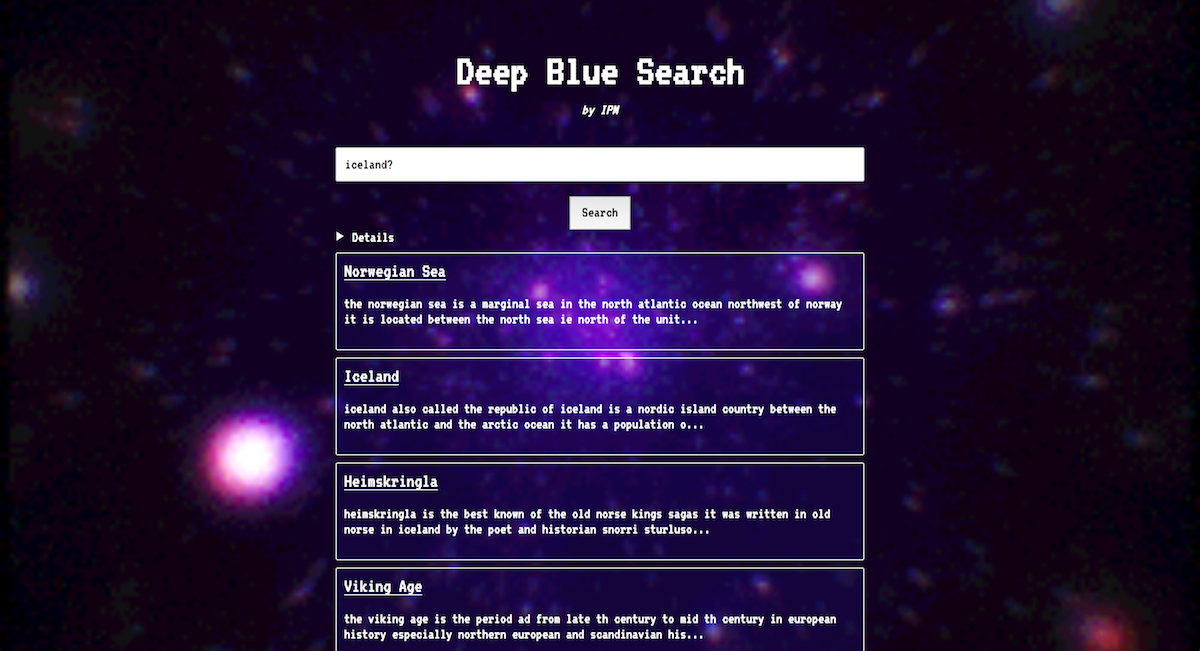
\includegraphics[width=\textwidth]{graphics/gui.png}
	\caption{The GUI after a search has been conducted}
	\label{fig:gui:results}
\end{figure}